\chapter{Diseño del sistema}


El presente capítulo describe el diseño del videojuego \textit{Ascension}. Se abordan la terminología del dominio, los requisitos funcionales expresados mediante historias de usuario, la propuesta arquitectónica del sistema y los patrones de diseño aplicados. El objetivo es proporcionar una visión completa de las decisiones de diseño antes de abordar la implementación detallada de los subsistemas.

\section{Terminología utilizada en este capítulo}


Antes de abordar los aspectos técnicos del desarrollo, se definen los términos específicos del dominio de los videojuegos y del motor Unity que se utilizan a lo largo de este capítulo:

\small
\begin{longtable}{|p{0.46\textwidth}|p{0.46\textwidth}|}
\hline
\textbf{Término} & \textbf{Definición} \\ \hline
\endfirsthead
\hline
\textbf{Término} & \textbf{Definición} \\ \hline
\endhead
\hline
\endfoot
\hline
\endlastfoot
\textit{Sprite} & Imagen bidimensional que representa visualmente un elemento del juego (personaje, enemigo, tile, objeto). En \textit{pixel art}, cada \textit{sprite} se compone de un número reducido de píxeles con colores definidos. \\ \hline
\textit{Tile} & Celda cuadrada de tamaño fijo que constituye la unidad básica de construcción de un nivel. Las salas de \textit{Ascension} se componen de tiles de $16 \times 16$ píxeles organizados en una rejilla. \\ \hline
\textit{Tilemap} & Rejilla bidimensional que almacena y renderiza tiles. Unity proporciona un componente \texttt{Tilemap} que gestiona automáticamente el posicionamiento y la visualización de los tiles. \\ \hline
\textit{Hitbox} & Área invisible asociada a un objeto del juego que define la zona en la que se detectan impactos. Cuando el \textit{hitbox} de un arma se superpone con el \textit{hitbox} de un enemigo, se registra un golpe. \\ \hline
\textit{Collider} & Componente de Unity que define la forma física de un objeto para la detección de colisiones. Un \texttt{BoxCollider2D} define un rectángulo; un \texttt{TilemapCollider2D} genera colisionadores automáticos a partir de los tiles de un \textit{tilemap}. \\ \hline
\textit{Trigger} & Modo especial de un \textit{collider} que detecta la superposición con otros objetos sin producir una respuesta física (sin empuje ni rebote). Se utiliza para detectar eventos como la entrada del jugador en una sala. \\ \hline
\textit{Prefab} & Plantilla reutilizable de un objeto del juego con todos sus componentes preconfigurados. Al instanciar un \textit{prefab}, se crea una copia independiente en la escena. \\ \hline
\textit{ScriptableObject} & Contenedor de datos de Unity que permite almacenar configuraciones (estadísticas de enemigos, datos de armas, efectos de tiles) como activos del proyecto, editables desde el inspector sin necesidad de modificar código. \\ \hline
\textit{Corutina} & Función de Unity que permite ejecutar código distribuido en múltiples fotogramas. Se utiliza para efectos temporales como el parpadeo de invulnerabilidad, el parpadeo rojo de muerte o la persistencia de efectos de tiles. \\ \hline
\texttt{Awake()} / \texttt{Start()} & Métodos del ciclo de vida de Unity que se ejecutan al inicializar un objeto. \texttt{Awake()} se llama al cargar el componente; \texttt{Start()} se ejecuta justo antes del primer fotograma. \\ \hline
\texttt{Update()} / \texttt{FixedUpdate()} & Métodos que Unity invoca de forma repetida. \texttt{Update()} se ejecuta una vez por fotograma (entrada y lógica general) y \texttt{FixedUpdate()} se ejecuta a intervalos fijos (física). \\ \hline
\texttt{Time.deltaTime} & Tiempo transcurrido desde el último fotograma. Se usa para que el movimiento y otros cálculos sean independientes de la tasa de fotogramas. \\ \hline
\texttt{Time.timeScale} & Factor que escala el tiempo del juego. Un valor cero detiene la simulación (útil para pausar); uno es tiempo normal. \\ \hline
\texttt{[SerializeField]} & Atributo de C\# usado en Unity para exponer un campo privado a configuración sin hacerlo público, permitiendo ajustar valores sin modificar código. \\ \hline
\texttt{Instantiate(...)} & Función que crea una instancia en tiempo de ejecución a partir de una plantilla (\textit{prefab}) u objeto existente. \\ \hline
\textit{Rigidbody2D} & Componente de física de Unity que aplica simulación física bidimensional a un objeto (gravedad, velocidad, colisiones). En \textit{Ascension} se utiliza con gravedad desactivada para movimiento cenital. \\ \hline
\texttt{DontDestroyOnLoad} & Método de Unity que impide que un objeto se destruya al cambiar de escena, permitiendo que gestores como \texttt{GameManager} persistan durante toda la ejecución. \\ \hline
\textit{Gizmos} & Elementos gráficos de depuración visibles únicamente durante el desarrollo (no en el juego final). Se utilizan para visualizar rangos de ataque, áreas de aparición y otros parámetros de diseño. \\ \hline
PPU (\textit{Pixels Per Unit}) & Número de píxeles del \textit{sprite} que equivalen a una unidad del mundo del juego. En \textit{Ascension}, el valor es dieciséis, lo que significa que un tile de $16 \times 16$ píxeles ocupa exactamente una unidad en el mundo. \\ \hline
\end{longtable}
\TablaTitulo{Glosario de términos técnicos utilizados en este capítulo.}


\section{Requisitos funcionales: historias de usuario}


La captura de requisitos funcionales se ha realizado mediante Historias de Usuario (HU), siguiendo la plantilla estándar del marco de trabajo ágil: \textit{«Como [rol], quiero [funcionalidad], para [beneficio]»}. Cada historia de usuario incluye criterios de aceptación verificables, una estimación en puntos de historia y una prioridad asignada. Las historias se han organizado por subsistemas funcionales.

Los criterios de aceptación se utilizan como especificación de requisitos. En el alcance del presente trabajo, su comprobación se ha realizado de forma manual durante el desarrollo mediante ejecución y observación en el editor de Unity, sin instrumentación específica para métricas de rendimiento ni una batería sistemática de casos de prueba automatizados.

\subsection{Sistema de combate}


\textbf{HU-001: Ataque cuerpo a cuerpo.}
\textit{Como} jugador, \textit{quiero} atacar enemigos con un arma cuerpo a cuerpo mediante un gesto de barrido, \textit{para} eliminar amenazas cercanas de forma intuitiva. Criterios de aceptación: el ataque se ejecuta al mantener presionado el botón izquierdo del ratón; el arma realiza un arco de 180 grados; existe un tiempo de espera de 0,5 segundos entre ataques; los enemigos dentro del área de impacto reciben daño; se muestra retroalimentación visual mediante un efecto de rastro. Prioridad: alta. Estimación: cinco puntos.

\textbf{HU-002: Ataque a distancia.}
\textit{Como} jugador, \textit{quiero} atacar enemigos desde una distancia segura disparando proyectiles, \textit{para} mantener una posición estratégica durante el combate. Criterios: el disparo se ejecuta al hacer clic con el botón izquierdo del ratón; el proyectil se dirige hacia la posición del cursor; existe un tiempo de espera de 0,3 segundos entre disparos; los proyectiles tienen un tiempo de vida de tres segundos; los proyectiles colisionan y se destruyen al impactar contra enemigos o muros. Prioridad: alta. Estimación: cinco puntos.

\textbf{HU-003: Sistema de daño.}
\textit{Como} jugador, \textit{quiero} que los enemigos muestren retroalimentación visual al ser golpeados, \textit{para} obtener información inmediata sobre la efectividad de los ataques. Criterios: el enemigo muestra un destello rojo de 0,1 segundos al recibir daño; la barra de vida se actualiza instantáneamente; el enemigo es destruido cuando su vida llega a cero; se otorga puntuación por cada eliminación. Prioridad: media. Estimación: tres puntos.

\textbf{HU-004: Recepción de daño del jugador.}
\textit{Como} jugador, \textit{quiero} experimentar un periodo de invulnerabilidad temporal tras recibir daño, \textit{para} disponer de tiempo para reaccionar y escapar de situaciones peligrosas. Criterios: el jugador recibe daño al colisionar con enemigos o proyectiles enemigos; se activa un periodo de invulnerabilidad de un segundo; durante la invulnerabilidad, el sprite parpadea en blanco a doce Hz; la interfaz de corazones se actualiza inmediatamente. Prioridad: alta. Estimación: cinco puntos.

\subsection{Sistema de movilidad}


\textbf{HU-005: Movimiento básico.}
\textit{Como} jugador, \textit{quiero} mover el personaje en ocho direcciones utilizando las teclas WASD, \textit{para} explorar las salas y esquivar ataques enemigos. Criterios: el movimiento responde a las teclas W, A, S, D; el personaje se mueve en las ocho direcciones cardinales e intercardinales; la velocidad se normaliza para evitar movimiento diagonal más rápido; el personaje no puede atravesar muros. Prioridad: crítica. Estimación: tres puntos.

\textbf{HU-006: Habilidad de esquiva (\textit{roll}).}
\textit{Como} jugador, \textit{quiero} realizar una esquiva rápida con invulnerabilidad temporal, \textit{para} evitar patrones de ataque enemigos. Criterios: la esquiva se activa con la tecla Espacio; el jugador se desplaza al doble de velocidad durante 0,4 segundos; durante la esquiva, el jugador es invulnerable a todo daño y atraviesa enemigos y proyectiles enemigos; existe un tiempo de espera de 0,6 segundos entre esquivas. Prioridad: alta. Estimación: cinco puntos.

\textbf{HU-007: Interacción con tiles de velocidad.}
\textit{Como} jugador, \textit{quiero} que la velocidad de movimiento se vea afectada por el tipo de suelo, \textit{para} añadir variabilidad táctica al posicionamiento. Criterios: los tiles de hielo incrementan la velocidad en un 50 \%; los tiles de lodo la reducen en un 50 \%; el efecto persiste durante cinco segundos tras abandonar el tile; los enemigos también se ven afectados. Prioridad: media. Estimación: cinco puntos.

\subsection{Sistema de progresión de salas}


\textbf{HU-008: Transición entre salas.}
\textit{Como} jugador, \textit{quiero} avanzar a la siguiente sala al derrotar a todos los enemigos e interactuar con las escaleras, \textit{para} progresar en la partida. Criterios: las escaleras se bloquean al entrar si hay enemigos; las escaleras se habilitan al derrotar a todos los enemigos; aparecen escaleras en una posición aleatoria de la sala; al presionar la tecla E sobre las escaleras se genera una nueva sala; la nueva sala presenta mayor dificultad. Prioridad: crítica. Estimación: ocho puntos.

\textbf{HU-009: Bloqueo de escaleras durante combate.}
\textit{Como} jugador, \textit{quiero} que las escaleras de la sala se bloqueen cuando hay enemigos activos, \textit{para} que cada combate deba completarse antes de avanzar. Criterios: las escaleras se bloquean automáticamente; se habilitan únicamente cuando todos los enemigos han sido eliminados. Prioridad: alta. Estimación: tres puntos.

\subsection{Sistema de enemigos}


\textbf{HU-010: Enemigos con inteligencia artificial diferenciada.}
\textit{Como} jugador, \textit{quiero} enfrentar enemigos con comportamientos diferenciados, \textit{para} experimentar variedad en los desafíos de combate. Criterios: existen tres arquetipos de enemigo (francotirador, perseguidor, saltador); cada arquetipo tiene un patrón de movimiento único; los enemigos no atacan inmediatamente tras aparecer (0,75 s de gracia); los enemigos respetan la física del entorno. Prioridad: crítica. Estimación: trece puntos.

\textbf{HU-011: Sistema de aparición de enemigos.}
\textit{Como} desarrollador, \textit{quiero} que los enemigos aparezcan de forma segura y equilibrada en cada sala, \textit{para} favorecer una experiencia de juego justa. Criterios: los enemigos nunca aparecen a menos de 2,5 unidades del jugador; el sistema realiza 25 intentos de posicionamiento antes de utilizar una posición de respaldo; el número de enemigos escala con la profundidad de la sala; se soportan modos de aparición por cantidad fija o por presupuesto de coste. Prioridad: alta. Estimación: ocho puntos.

\textbf{HU-012: Variantes de slimes.}
\textit{Como} jugador, \textit{quiero} que cada tipo de slime tenga un color y comportamiento distintivo, \textit{para} poder anticipar sus patrones de ataque. Criterios: el slime verde mantiene distancia y dispara proyectiles; el slime rojo persigue al jugador para daño por contacto; el slime azul realiza saltos rápidos hacia el jugador; cada slime tiene sprites únicos. Prioridad: media. Estimación: ocho puntos.

\subsection{Sistema de progresión y puntuación}


\textbf{HU-013: Sistema de puntuación.}
\textit{Como} jugador, \textit{quiero} acumular puntos por los logros durante la partida. Criterios: 100 puntos por sala completada; puntos variables por enemigo eliminado (daño del enemigo $\times 5$); 1.000 puntos de bonificación por completar el juego. Prioridad: media. Estimación: tres puntos.

\textbf{HU-014: Historial de partidas.}
\textit{Como} jugador, \textit{quiero} ver un registro de las mejores partidas anteriores. Criterios: el historial almacena hasta 30 partidas; cada entrada muestra puntuación, clase, salas, enemigos, resultado y fecha; los datos persisten entre sesiones de juego; se puede limpiar el historial desde el menú principal. Prioridad: baja. Estimación: cinco puntos.

\textbf{HU-015: Sistema de clases de personaje.}
\textit{Como} jugador, \textit{quiero} elegir entre diferentes clases de personaje con estadísticas únicas. Criterios: cada clase tiene estadísticas diferenciadas (vida, velocidad); cada clase comienza con un arma inicial específica; la selección se realiza en una escena dedicada. Prioridad: media. Estimación: cinco puntos.

\textbf{HU-016: Tiles de potenciación.}
\textit{Como} jugador, \textit{quiero} encontrar tiles especiales que mejoren temporalmente las capacidades del personaje. Criterios: los tiles de potenciación aumentan el daño en +1 durante cinco segundos; los tiles de curación restauran un punto de vida; el efecto se aplica a todas las armas y proyectiles; los efectos se reinician al cambiar de sala. Prioridad: media. Estimación: cinco puntos.

\subsection{Sistema de generación procedural}


\textbf{HU-017: Generación aleatoria de salas.}
\textit{Como} jugador, \textit{quiero} que cada sala se genere de forma diferente en cada partida. Criterios: cada sala tiene un tamaño base de $26 \times 12$ tiles; el suelo se compone de tiles normales y especiales distribuidos aleatoriamente; los muros forman un perímetro cerrado con colisionadores funcionales; la generación completa requiere menos de 100 ms. Prioridad: crítica. Estimación: trece puntos.

\textbf{HU-018: Distribución de tiles especiales.}
\textit{Como} desarrollador, \textit{quiero} controlar la rareza y distribución de tiles especiales, \textit{para} equilibrar la dificultad. Criterios: tiles de hielo y lodo aparecen en manchas de 4-9 tiles con un 12 \% de probabilidad; tiles de potenciación aparecen individualmente con un 18 \% de probabilidad (1-2 por sala); tiles de curación son extremadamente raros (2 \% de probabilidad, máximo uno por sala). Prioridad: media. Estimación: ocho puntos.

\textbf{HU-019: Sistema de variantes de tiles.}
\textit{Como} jugador, \textit{quiero} ver variedad visual en los tiles del suelo. Criterios: cada tipo de tile tiene múltiples sprites alternativos; la selección es determinista basada en la posición; se soportan hasta diez variantes por tipo de tile. Prioridad: baja. Estimación: cinco puntos.

\subsection{Sistema de interfaz de usuario}


\textbf{HU-020: Representación de vida mediante corazones.}
\textit{Como} jugador, \textit{quiero} ver la vida actual representada mediante corazones en la interfaz. Criterios: cada corazón representa un punto de vida; la cantidad se ajusta dinámicamente según la clase seleccionada; la representación se actualiza instantáneamente al recibir o curar daño. Prioridad: alta. Estimación: cinco puntos.

\textbf{HU-021: Menú de pausa.}
\textit{Como} jugador, \textit{quiero} poder pausar el juego en cualquier momento. Criterios: el menú se abre y cierra con la tecla ESC; el tiempo del juego se detiene (\texttt{Time.timeScale = 0}); se muestran opciones de reanudar y menú principal. Prioridad: alta. Estimación: tres puntos.

\textbf{HU-022: Pantallas de fin de partida.}
\textit{Como} jugador, \textit{quiero} ver una pantalla específica al morir o ganar, \textit{para} confirmar el final de la partida. Criterios: se muestra una pantalla de derrota o de victoria; las estadísticas se registran automáticamente en el historial. Prioridad: media. Estimación: cinco puntos.

\subsection{Historias técnicas}


\textbf{HT-001: Sistema de persistencia.} Implementación de persistencia de datos mediante \texttt{PlayerPrefs} para datos simples y serialización JSON para estructuras complejas, con validación de datos al cargar y límite de 30 entradas en el historial. Prioridad: media. Estimación: cinco puntos.

\textbf{HT-002: Optimización de rendimiento.} Uso de almacenamiento en caché de componentes en \texttt{Awake()} para evitar llamadas a \texttt{GetComponent} en \texttt{Update()}; uso selectivo de \texttt{CollisionDetectionMode2D}\texttt{.Continuous}; minimización de búsquedas \texttt{GameObject.Find}. Prioridad: media. Estimación: ocho puntos.

\textbf{HT-003: Sistema de registro y depuración.} Implementación de mensajes de advertencia para configuraciones incorrectas, registros informativos en transiciones críticas de estado, y visualización de \textit{Gizmos} durante el desarrollo para rangos de enemigos. Prioridad: baja. Estimación: tres puntos.

\section{Propuesta arquitectónica}


\subsection{Visión general de la arquitectura}


La arquitectura del sistema se fundamenta en el paradigma de programación orientada a componentes proporcionado por Unity Engine, combinado con patrones de diseño de la ingeniería del software clásica (\textit{Singleton}, \textit{Observer}, \textit{Strategy}, \textit{Template Method}). Se seleccionó esta combinación frente a una arquitectura puramente basada en herencia porque el sistema de componentes de Unity favorece la composición: cada entidad del juego se define como un \texttt{GameObject} al que se agregan componentes independientes, lo que permite reutilizar funcionalidades sin crear jerarquías de herencia profundas. Los patrones de diseño complementan esta arquitectura proporcionando soluciones probadas para problemas recurrentes -- acceso global a gestores (\textit{Singleton}), desacoplamiento entre lógica y presentación (\textit{Observer}), intercambiabilidad de algoritmos (\textit{Strategy}) y reutilización de comportamiento base (\textit{Template Method}) -- que el sistema de componentes por sí solo no resuelve.

La estructura resultante se organiza en dos capas diferenciadas:

\begin{itemize}
\item \textbf{Capa de lógica de juego.} Contiene los componentes que implementan las reglas del juego: \texttt{GameManager} (máquina de estados y progresión), \texttt{RoomFlowController} (secuenciación de salas), \texttt{RoomGenerator} (generación procedural de tiles y muros), \texttt{EnemyManager} (aparición y seguimiento de enemigos), \texttt{PlayerController} (movimiento en ocho direcciones y esquiva), \texttt{PlayerHealth} (gestión de puntos de vida e invulnerabilidad), la jerarquía de enemigos (\texttt{Enemy}, \texttt{SlimeGreen}, \texttt{SlimeRed}, \texttt{SlimeBlue}) y el sistema de armas (\texttt{Weapon}, \texttt{MeleeWeapon}, \texttt{RangedWeapon}, \texttt{Projectile}). En términos generales, se evita que esta capa dependa directamente de la interfaz de usuario; cuando se requiere una actualización visual inmediata y acotada (por ejemplo, la vida en corazones), se utiliza una referencia explícita a un componente de presentación.
\item \textbf{Capa de presentación.} Contiene los componentes de interfaz: \texttt{HeartDisplay} (visualización de vida mediante iconos de corazones), \texttt{ScoreDisplay} (puntuación en tiempo real), \texttt{PauseMenu} (menú de pausa con opciones de navegación), \texttt{GameOverScreen} y \texttt{VictoryScreen} (pantallas de fin de partida con estadísticas), y \texttt{ScoreboardMenuUI} (historial de puntuaciones con hasta treinta entradas). Estos componentes se suscriben a eventos emitidos por la capa de lógica y reaccionan a los cambios de estado sin que la capa de lógica conozca su existencia.
\end{itemize}

La comunicación entre ambas capas se realiza principalmente mediante el patrón \textit{Observer}: los gestores centrales (\textit{managers}) exponen eventos C\# (definidos mediante delegados con nombre) a los que los componentes de presentación se suscriben durante su inicialización. Por ejemplo, cuando el \texttt{GameManager} cambia su estado a \texttt{Paused}, emite el evento \texttt{OnGameStateChanged}; el \texttt{PauseMenu}, suscrito a este evento, activa su panel de interfaz y la escala de tiempo del juego se detiene. Para actualizaciones de interfaz muy concretas y de baja complejidad -- como la visualización de corazones -- se emplea una referencia directa (\texttt{PlayerHealth} -> \texttt{HeartDisplay}) por simplicidad, evitando introducir infraestructura de eventos adicional para un caso puntual.

\begin{figure}[H]
\begin{center}
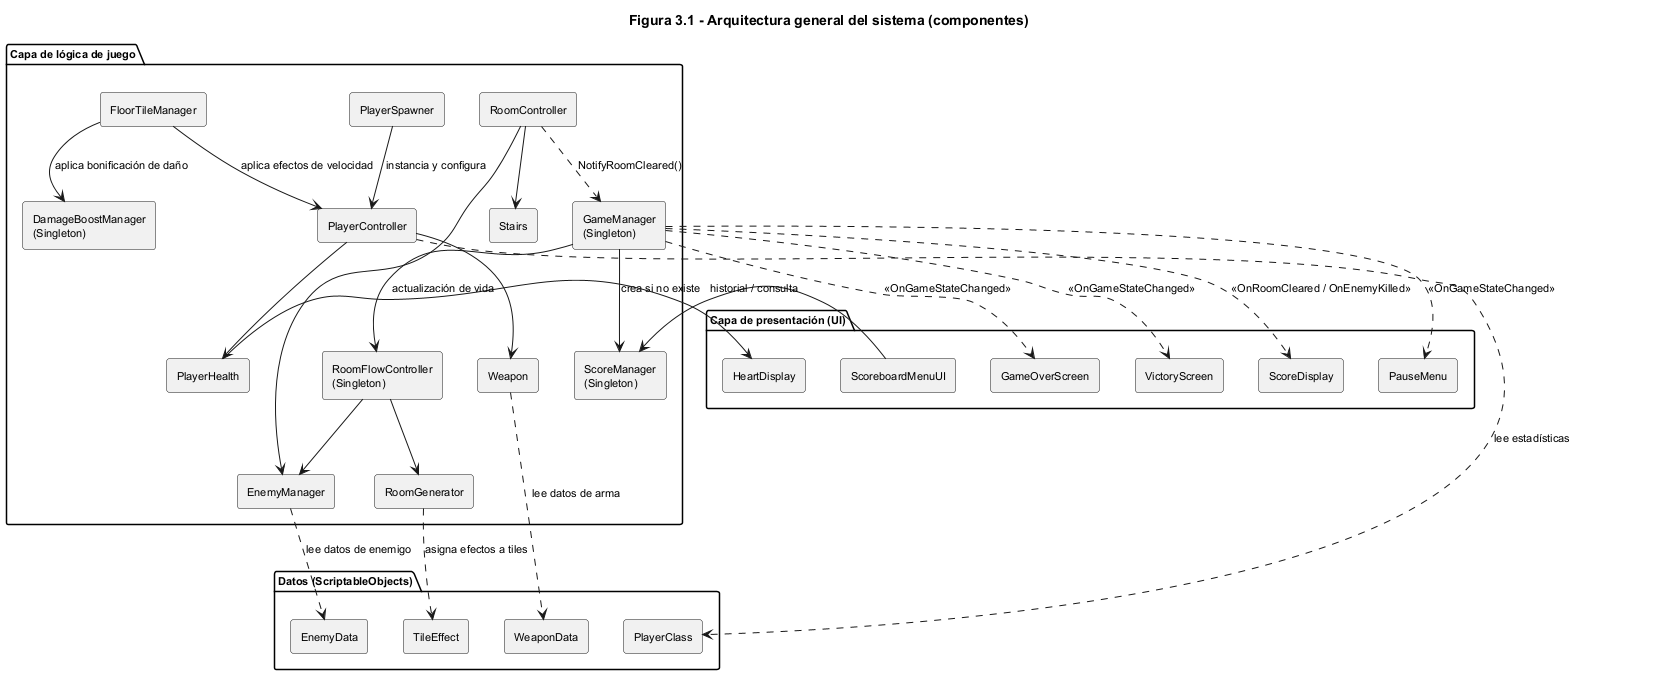
\includegraphics[width=0.95\textwidth]{Figuras/figura3_1_arquitectura_componentes.png}
\caption{
Diagrama de componentes de la arquitectura general del sistema. \textit{Elaboración propia.}
}
\label{fig:placeholder-1}
\end{center}
\end{figure}


\subsection{Flujo de escenas}


El proyecto se estructura en tres escenas de Unity que representan las fases del flujo de juego:

\begin{enumerate}
\item \textbf{MainMenu.} Escena del menú principal, con opciones para iniciar partida, consultar el historial de puntuaciones y salir del juego.
\item \textbf{ClassSelection.} Escena de selección de clase de personaje, donde el jugador elige entre las clases disponibles antes de comenzar la partida.
\item \textbf{GameScene.} Escena principal del juego, donde se desarrolla toda la acción. La generación procedural de salas se realiza dentro de esta misma escena, regenerando el contenido del \textit{tilemap} sin necesidad de cargar escenas adicionales.
\end{enumerate}

\begin{figure}[H]
\begin{center}
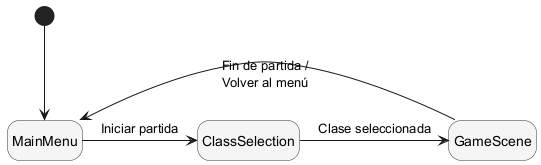
\includegraphics[width=0.95\textwidth]{Figuras/flujo_escenas_simple.png}
\caption{
Diagrama del flujo de escenas. \textit{Elaboración propia.}
}
\label{fig:placeholder-2}
\end{center}
\end{figure}


\subsection{Gestores centrales (\textit{managers})}


El sistema utiliza cuatro gestores centrales que implementan el patrón \textit{Singleton}. Tres de ellos (\texttt{GameManager}, \texttt{ScoreManager} y \texttt{DamageBoostManager}) persisten entre cambios de escena mediante \texttt{DontDestroyOnLoad} (directiva que evita que Unity destruya el objeto al cargar otra escena); el \texttt{RoomFlowController} opera como \textit{Singleton} de escena, re-instanciándose en cada escena de juego y re-enlazándose a los componentes necesarios mediante el evento \texttt{SceneManager.sceneLoaded}:

\begin{table}[H]
\begin{center}
\small
\begin{tabular}{|p{0.46\textwidth}|p{0.46\textwidth}|}
\hline
Gestor & Responsabilidad \\ \hline
\texttt{GameManager} & Control de estados del juego, progresión, transiciones entre escenas \\ \hline
\texttt{ScoreManager} & Cálculo de puntuación, persistencia del historial de partidas \\ \hline
\texttt{RoomFlowController} & Control del bucle de generación y progresión de salas \\ \hline
\texttt{DamageBoostManager} & Gestión de bonificaciones temporales de daño \\ \hline
\end{tabular}
\end{center}
\end{table}


\TablaTitulo{Gestores centrales del sistema.}

\subsection{Diagrama de dependencias}


La estructura de dependencias entre los módulos principales del sistema se organiza de la siguiente forma. El diagrama muestra la relación jerárquica entre componentes: cada nodo depende de los nodos situados debajo de él en la jerarquía. Las flechas indican dependencias de creación, referencia directa o suscripción a eventos. Los nodos marcados con \textit{(ScriptableObject)} representan activos de datos configurables desde el inspector de Unity.

\begin{figure}[H]
\begin{center}
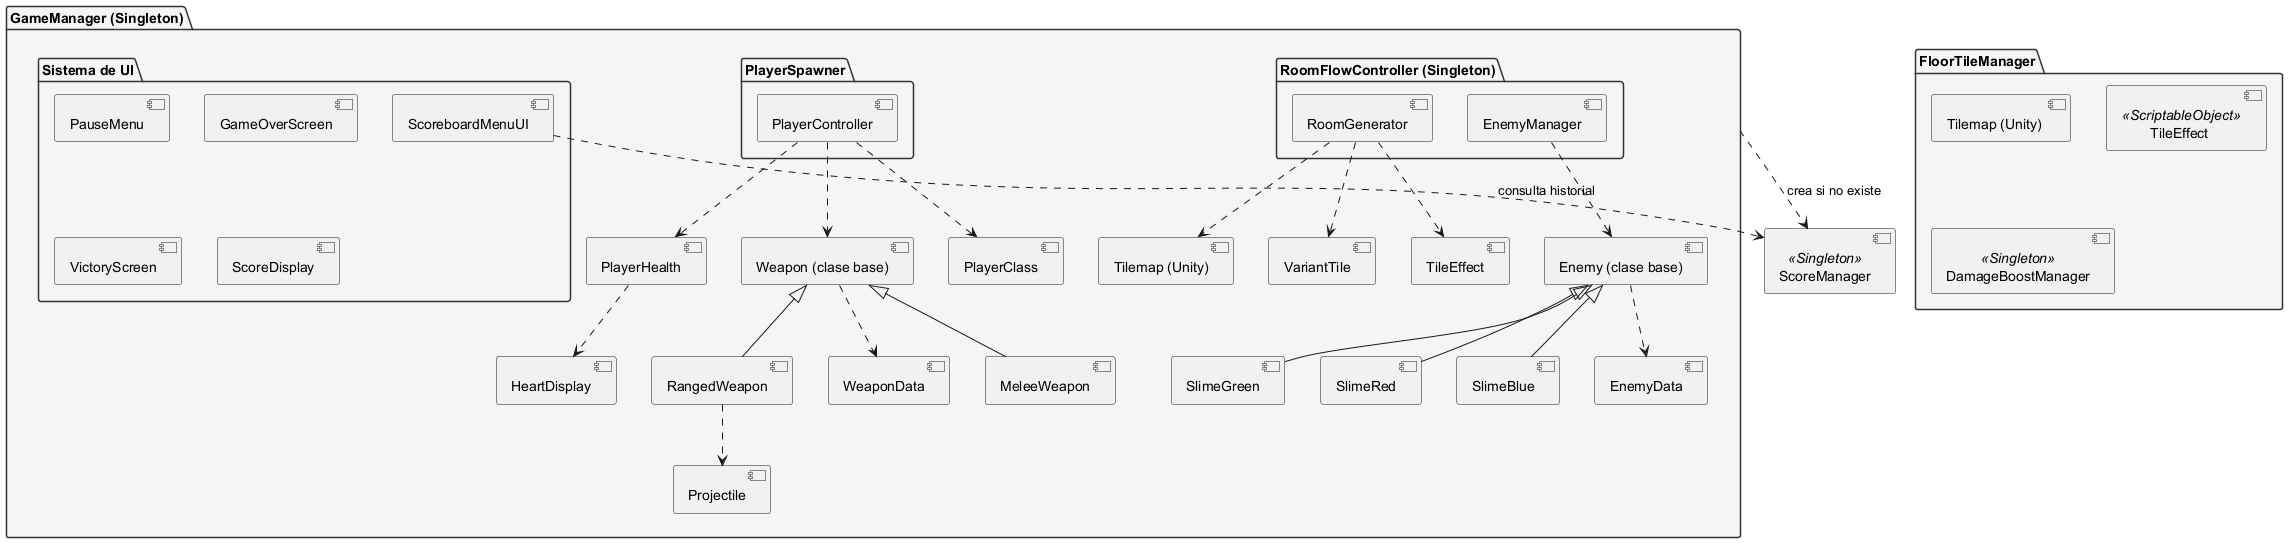
\includegraphics[width=0.95\textwidth]{Figuras/dependencias_modulos.png}
\caption{
Diagrama de dependencias entre los módulos del sistema. \textit{Elaboración propia.}
}
\label{fig:placeholder-4}
\end{center}
\end{figure}


\subsection{Flujo de producción: del activo gráfico al juego}


Esta sección describe el proceso completo de producción seguido para transformar los activos gráficos (\textit{sprites}) en entidades funcionales dentro del juego. El flujo abarca desde la creación e importación de los \textit{sprites} hasta la configuración de los \textit{GameObjects} con sus componentes de física, colisión y animación, y su posterior ensamblaje en la escena del juego.

\subsubsection{Importación y configuración de \textit{sprites}}


Los activos gráficos del proyecto se crearon en LibreSprite como \textit{pixel art} a resoluciones de 16x16, 32x32 y 64x64 píxeles, según el tipo de elemento (tiles, personajes y enemigos, respectivamente). Tras la exportación en formato PNG, la importación en Unity requiere una configuración específica para preservar la estética del \textit{pixel art}:

\begin{itemize}
\item \textbf{Pixels Per Unit (PPU):} se establece en 16 para que cada tile de 16x16 píxeles ocupe exactamente una unidad del mundo del juego. Esta correspondencia simplifica el cálculo de posiciones en el \textit{tilemap} y garantiza la coherencia entre la cuadrícula de tiles y las coordenadas del sistema de física.
\item \textbf{Filtrado:} se configura como \textit{Point (no filter)} para evitar el suavizado de bordes entre píxeles, preservando la apariencia nítida del \textit{pixel art}.
\item \textbf{Compresión:} se desactiva o se establece en modo sin pérdida (\textit{None}) para evitar artefactos visuales que distorsionarían los bordes de los \textit{sprites}.
\item \textbf{Modo de \textit{sprite}:} para personajes y enemigos con múltiples fotogramas de animación, se utiliza el modo \textit{Multiple}, que permite particionar una hoja de \textit{sprites} (\textit{spritesheet}) en fotogramas individuales mediante el editor de \textit{sprites} de Unity.
\end{itemize}

\begin{figure}[H]
\begin{center}
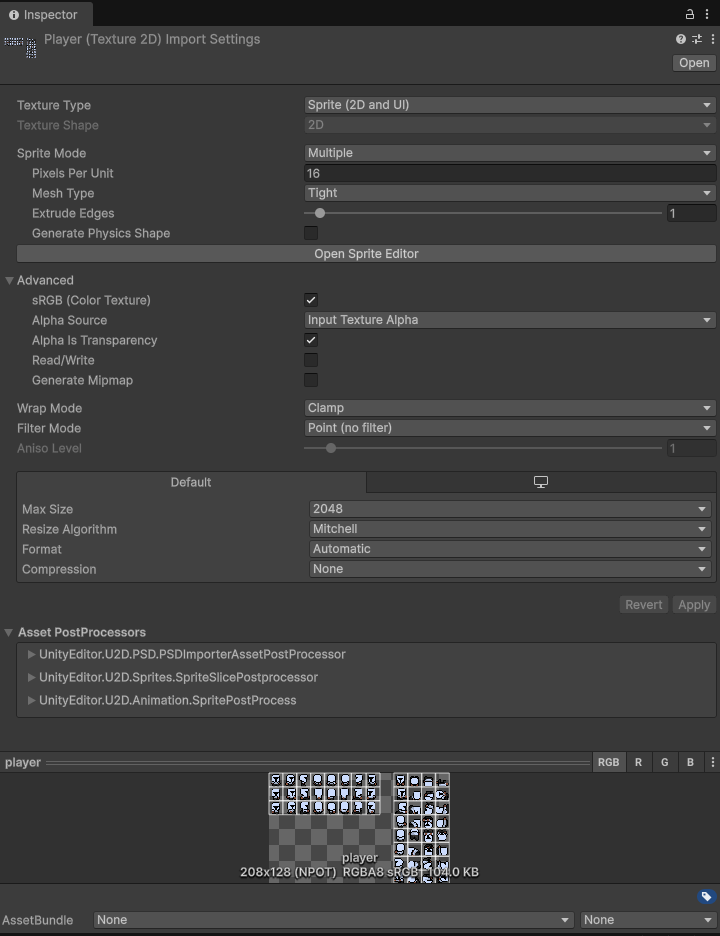
\includegraphics[width=0.9\textwidth]{Figuras/captura_9.png}
\caption{Configuración de importación de un \textit{sprite} en el inspector de Unity, mostrando los parámetros PPU, filtrado y compresión. \textit{Elaboración propia.}}
\label{fig:placeholder-6}
\end{center}
\end{figure}


\subsubsection{Creación de \textit{GameObjects} y configuración de componentes}


Cada entidad del juego se construye como un \textit{GameObject} de Unity al que se agregan los componentes necesarios para su funcionamiento. A continuación se describe la configuración típica para los principales tipos de entidad.

\textbf{Jugador:}
\begin{itemize}
\item \texttt{SpriteRenderer}: renderiza el \textit{sprite} del personaje con el orden de capa adecuado.
\item \texttt{Rigidbody2D}: habilita la simulación física con gravedad desactivada (movimiento cenital), detección de colisiones continua y rotación congelada.
\item \texttt{CircleCollider2D}: define el área física del personaje para la detección de colisiones con muros y enemigos. Se ha usado un colisionador circular en la zona central y desplazado hacia abajo para que las colisiones con muros sean más naturales (evitando que el jugador pueda quedar atrapado por colisionadores rectangulares en esquinas o bordes).
\item \texttt{PlayerController} (script): gestiona el movimiento y la esquiva.
\item \texttt{PlayerHealth} (script): gestiona los puntos de vida y la invulnerabilidad.
\item \texttt{Animator}: controla las transiciones entre estados de animación (reposo, movimiento, esquiva, daño).
\end{itemize}

\begin{figure}[H]
\begin{center}
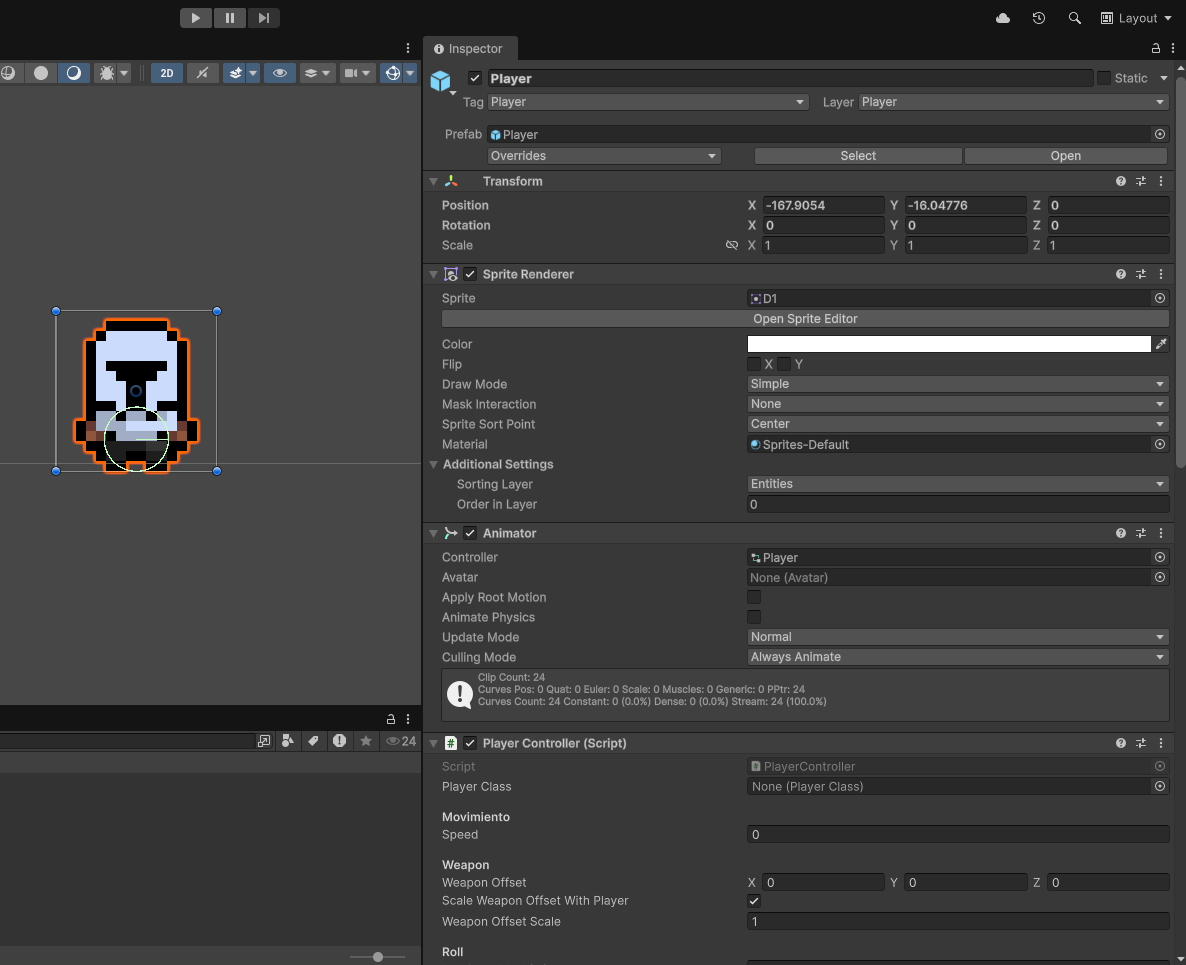
\includegraphics[width=0.9\textwidth]{Figuras/captura_10.png}
\caption{Vista del inspector de Unity mostrando los componentes configurados en el \textit{GameObject} del jugador: \textit{SpriteRenderer}, \textit{Rigidbody2D}, \textit{CircleCollider2D}, scripts y \textit{Animator}. \textit{Elaboración propia.}}
\label{fig:placeholder-7}
\end{center}
\end{figure}


\textbf{Enemigo (ejemplo: Slime Verde):}
\begin{itemize}
\item \texttt{SpriteRenderer}: renderiza el \textit{sprite} del enemigo.
\item \texttt{Rigidbody2D}: física 2D sin gravedad, con detección de colisiones continua.
\item \texttt{CircleCollider2D}: define el área de contacto del enemigo. Se utiliza un colisionador circular en lugar de rectangular porque la forma redondeada del \textit{slime} produce colisiones más naturales al contacto con el jugador y con los muros.
\item \texttt{SlimeGreen} (script): implementa la IA del enemigo francotirador.
\item \texttt{Animator}: gestiona las animaciones de movimiento, ataque y muerte.
\end{itemize}

\begin{figure}[H]
\begin{center}
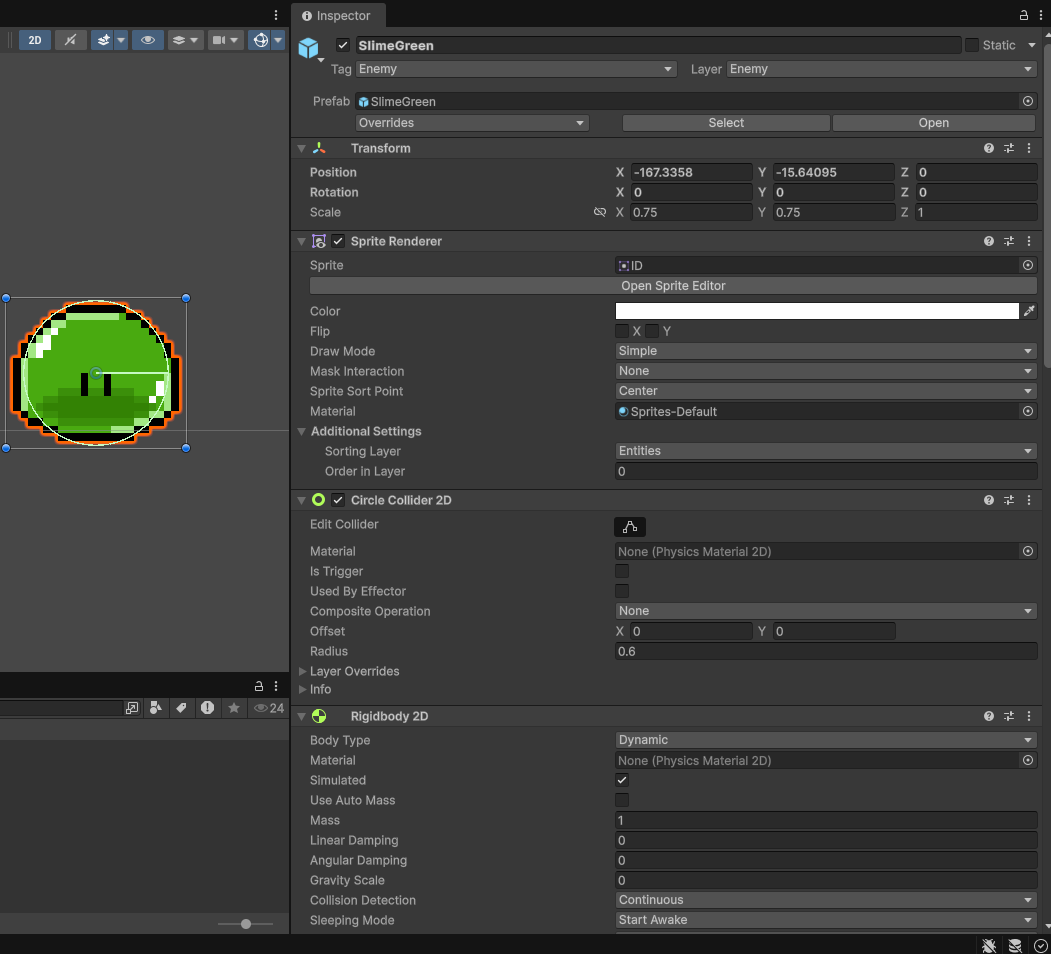
\includegraphics[width=0.9\textwidth]{Figuras/captura_11.png}
\caption{Vista del inspector de Unity mostrando los componentes de un enemigo \textit{Slime Verde}, con detalle del \textit{CircleCollider2D} y sus dimensiones. \textit{Elaboración propia.}}
\label{fig:placeholder-8}
\end{center}
\end{figure}


\subsubsection{Configuración de \textit{colliders} y \textit{hitboxes}}


La detección de colisiones se organiza en dos categorías:

\begin{itemize}
\item \textbf{\textit{Colliders} físicos} (modo no \textit{trigger}): producen respuesta física (empuje, bloqueo). Se utilizan en los muros perimetrales de las salas (\texttt{TilemapCollider2D} + \texttt{CompositeCollider2D} en el \textit{tilemap} de muros) y en el cuerpo del jugador y los enemigos, impidiendo que atraviesen paredes u otros objetos sólidos.
\item \textbf{\textit{Colliders de tipo trigger}} (modo \textit{Is Trigger} activado): detectan superposición sin respuesta física. Se utilizan para la detección de impactos de armas cuerpo a cuerpo (el \textit{hitbox} del arma), la detección de proyectiles contra enemigos o muros, la activación de escaleras al presionar la tecla de interacción y la detección de tiles especiales bajo el jugador o los enemigos.
\end{itemize}

La configuración del \textit{TilemapCollider2D} resulta especialmente relevante para la generación procedural. Al añadir un componente \texttt{TilemapCollider2D} al \textit{tilemap} de muros, Unity genera automáticamente un colisionador por cada tile presente en ese \textit{tilemap}. Combinado con un \texttt{CompositeCollider2D}, los colisionadores individuales se fusionan en un único colisionador perimetral continuo, lo que reduce el coste computacional de la simulación física y evita que el jugador pueda deslizarse entre los bordes de tiles adyacentes.

\subsubsection{Configuración de \textit{tilemaps} y tiles}


El sistema de niveles se construye sobre dos \textit{tilemaps} de Unity superpuestos en la misma escena:

\begin{enumerate}
\item \textbf{Tilemap de muros} (\texttt{wallTilemap}): contiene los tiles de muro que forman el perímetro de cada sala. Incluye los componentes \texttt{TilemapCollider2D} y \texttt{CompositeCollider2D} para generar la barrera física.
\item \textbf{Tilemap de suelo} (\texttt{floorTilemap}): contiene los tiles de suelo (normales y especiales) que componen el área jugable. No genera colisionadores, ya que el suelo no bloquea el movimiento.
\end{enumerate}

Cada tile se configura como un activo de tipo \texttt{VariantTile} (clase derivada de \texttt{TileBase} de Unity) que almacena múltiples variantes visuales del mismo tipo de tile. Al colocar un tile, el sistema selecciona una variante de forma determinista según la posición, lo que produce variabilidad visual sin aleatorización explícita.

\begin{figure}[H]
\begin{center}
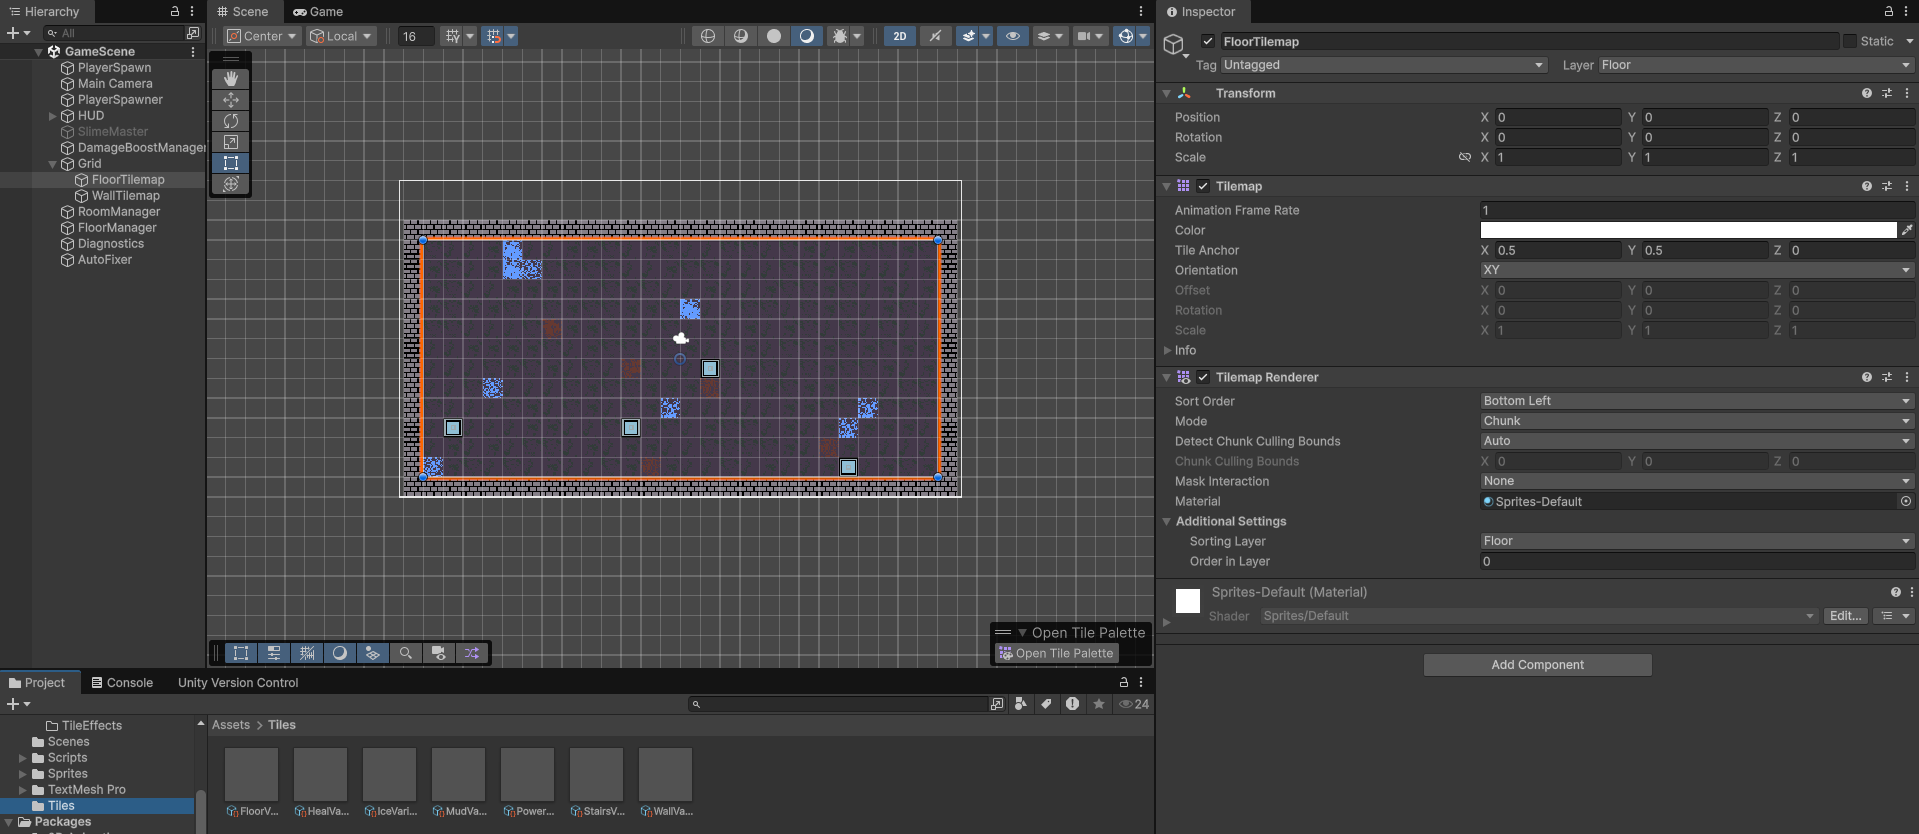
\includegraphics[width=0.9\textwidth]{Figuras/captura_12.png}
\caption{Editor de \textit{tilemaps} de Unity mostrando las dos capas (muros y suelo). \textit{Elaboración propia.}}
\label{fig:placeholder-10}
\end{center}
\end{figure}


\subsubsection{Sistema de animaciones}


Las animaciones del juego se implementan mediante el sistema de animación de Unity (\texttt{Animator} + \texttt{AnimationClip}). Cada personaje y enemigo dispone de un controlador de animación (\texttt{Animator Controller}) que define los estados de animación posibles y las transiciones entre ellos.

Para el jugador, los estados de animación incluyen:
\begin{itemize}
\item \textbf{Reposo} (\textit{idle}): animación cíclica de dos fotogramas con cadencia lenta.
\item \textbf{Movimiento} (\textit{walk}): animación cíclica de cuatro fotogramas. La dirección del movimiento (arriba, abajo, izquierda, derecha) se controla mediante parámetros del \textit{Animator} (\texttt{moveX}, \texttt{moveY}), lo que permite seleccionar la animación correspondiente a la dirección actual sin necesidad de un \textit{blend tree} completo.
\item \textbf{Esquiva} (\textit{roll}): animación de tres fotogramas que se reproduce una vez durante la duración de la esquiva.
\end{itemize}

Para los enemigos, los estados de animación incluyen reposo, movimiento y muerte, con transiciones controladas por parámetros del \textit{Animator} que los scripts de IA actualizan en cada fotograma.

\begin{figure}[H]
\begin{center}
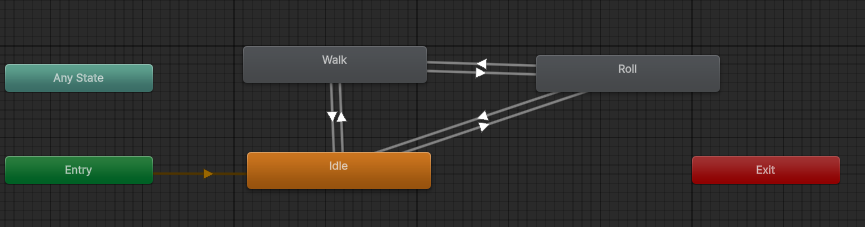
\includegraphics[width=0.9\textwidth]{Figuras/captura_13.png}
\caption{Controlador de animación (\textit{Animator Controller}) del jugador en Unity, mostrando los estados y las transiciones entre animaciones de reposo, movimiento y esquiva. \textit{Elaboración propia.}}
\label{fig:placeholder-11}
\end{center}
\end{figure}


\subsubsection{De los componentes al flujo de juego}


Una vez configurados los \textit{GameObjects} individuales con sus componentes, el flujo de juego se construye mediante la coordinación de estos elementos:

\begin{enumerate}
\item El \texttt{PlayerSpawner} instancia el \textit{prefab} del jugador en la posición inicial de la sala.
\item El \texttt{RoomGenerator} genera la estructura de tiles de la sala sobre los dos \textit{tilemaps} (muros y suelo).
\item El \texttt{EnemyManager} instancia los \textit{prefabs} de los enemigos en posiciones seguras dentro de la sala.
\item El \texttt{RoomFlowController} coordina la secuencia: bloqueo de escaleras -> combate -> habilitación de escaleras -> interacción -> siguiente sala.
\item El \texttt{GameManager} supervisa el estado global y gestiona las transiciones entre menú, juego, pausa, victoria y derrota.
\end{enumerate}

Cada \textit{prefab} contiene la configuración completa de su \textit{GameObject} (componentes, valores de campos serializados, referencias a \textit{ScriptableObjects}), de modo que al instanciarlo se obtiene una copia funcional del elemento sin necesidad de configuración adicional en tiempo de ejecución.


\section{Patrones y mecanismos de diseño aplicados}


En el apartado de estado del arte se presentaron los patrones de diseño seleccionados para el proyecto y la fundamentación teórica de cada uno. En este apartado se describe su aplicación concreta en la arquitectura de \textit{Ascension}: para cada patrón se presenta el código resultante y se analizan los detalles de implementación específicos del proyecto.

\subsection{Patrón \textit{Singleton}}


Como se fundamentó en el apartado correspondiente del estado del arte, el patrón \textit{Singleton} se seleccionó para los cuatro gestores centrales frente a la inyección de dependencias. Los tres gestores persistentes (\texttt{GameManager}, \texttt{ScoreManager}, \texttt{DamageBoostManager}) comparten la siguiente estructura:

\begin{lstlisting}
public static GameManager Instance { get; private set; }

void Awake() {
    if (Instance == null) {
        Instance = this;
        DontDestroyOnLoad(gameObject);
    } else {
        Destroy(gameObject);
    }
}
\end{lstlisting}


El \texttt{RoomFlowController} aplica la misma estructura de instancia única, pero omite \texttt{DontDestroy-}\texttt{OnLoad} porque sus referencias a componentes de escena (\texttt{RoomGenerator}, \texttt{EnemyManager}, \texttt{Tilemap}) se invalidan al cambiar de escena; en su lugar, se re-instancia en cada escena de juego y reconstruye sus referencias en el evento \texttt{SceneManager.sceneLoaded}.

\subsection{Patrón \textit{Observer}}


Como se describió en el análisis de patrones del estado del arte, el patrón \textit{Observer} desacopla el \texttt{GameManager} de los componentes de interfaz. Su implementación concreta utiliza los eventos \texttt{OnGameStateChanged}, \texttt{OnRoomCleared} y \texttt{OnEnemyKilled}:

\begin{lstlisting}
// En GameManager (emisor)
public delegate void GameStateChanged(GameState newState);
public static event GameStateChanged OnGameStateChanged;

// En PauseMenu (receptor)
void Start() {
    EnsureRuntimeUIIfMissing();
    WireButtonsOnce();
    GameManager.OnGameStateChanged += OnGameStateChanged;
}

private void OnGameStateChanged(GameState newState) {
    EnsureRuntimeUIIfMissing();
    if (pauseMenuPanel == null) return;
    pauseMenuPanel.SetActive(newState == GameState.Paused);
}
\end{lstlisting}


El \texttt{GameManager} desconoce cuántos ni cuáles componentes están suscritos, lo que permite añadir nuevos componentes reactivos (por ejemplo, un sistema de audio que reproduzca un efecto al completar una sala) sin modificar el código del gestor.

\subsection{Patrón \textit{Strategy}}


Como se describió en el análisis de patrones, el patrón \textit{Strategy} estructura el sistema de armas mediante subclases especializadas de \texttt{Weapon}. Cada tipo requiere campos específicos distintos (\texttt{swingAngle} para melee, \texttt{bulletPrefab} para ranged), lo que confirma la decisión de evitar condicionales internos:

\begin{lstlisting}
// Weapon es una clase concreta con Attack() virtual (cuerpo vacio);
// las subclases lo sobrescriben con su propio comportamiento.
public class Weapon : MonoBehaviour {
    public virtual void Attack() { }   // no-op de forma predeterminada
}

public class MeleeWeapon : Weapon {
    public override void Attack() {
        // Ataque de barrido con hitbox
    }
}

public class RangedWeapon : Weapon {
    public override void Attack() {
        // Disparo de proyectil
    }
}
\end{lstlisting}


El \texttt{PlayerController} interactúa con cualquier arma a través de la interfaz común \texttt{Weapon.Attack()}, sin necesidad de conocer el tipo concreto. Añadir un nuevo tipo de arma solo requiere crear una nueva subclase sin modificar el código existente.

\subsection{Patrón \textit{Template Method}}


Como se describió en el análisis de patrones, el patrón \textit{Template Method} estructura la jerarquía de enemigos. Sin este patrón, las alternativas serían: (a) tres clases independientes duplicando $\sim$180 líneas de lógica común, o (b) una única clase de $\sim$800 líneas con condicionales \texttt{switch(enemyType)}:

\begin{lstlisting}
public class Enemy : MonoBehaviour {
    protected virtual void Start() {
        // Inicializacion base: vida, fisica, gracia
    }
    
    protected virtual void Update() {
        // Logica base: verificacion de gracia, efectos de tiles
    }
    
    protected virtual void Die() {
        // Muerte base: notificacion, animacion, destruccion
    }
}

public class SlimeGreen : Enemy {
    protected override void Update() {
        base.Update();
        // Logica especifica: evaluar distancia, disparar
    }
}
\end{lstlisting}


La clase base \texttt{Enemy} define el esqueleto de comportamiento común (gestión de vida, detección de contacto, muerte, interacción con tiles), mientras que cada subclase especializa únicamente la inteligencia artificial, permitiendo añadir nuevos tipos de enemigo sin modificar las clases existentes.

\subsection{Arquitectura basada en componentes (Entidad-Componente)}


Además de los patrones clásicos, el análisis del estado del arte introdujo la arquitectura de componentes de Unity. Su aplicación en \textit{Ascension} responde al siguiente problema:

\textbf{Problema.} Las entidades del juego (jugador, enemigos, proyectiles) requieren combinaciones variables de funcionalidades: un enemigo necesita física, renderizado y lógica de IA, pero no control de entrada; el jugador necesita control de entrada, física, vida y arma, pero no lógica de IA.

\textbf{Alternativa descartada.} Herencia múltiple de una jerarquía profunda (\texttt{Entity > MovableEntity > DamageableEntity > PlayerEntity}). Se descartó porque C\# no soporta herencia múltiple y porque las jerarquías profundas producen clases base sobrecargadas con funcionalidad que no todas las subclases necesitan (el denominado \textit{fragile base class problem}).

\textbf{Aplicación en el proyecto:} Toda la arquitectura del juego se fundamenta en la composición de componentes proporcionada por Unity.

\begin{figure}[H]
\begin{center}
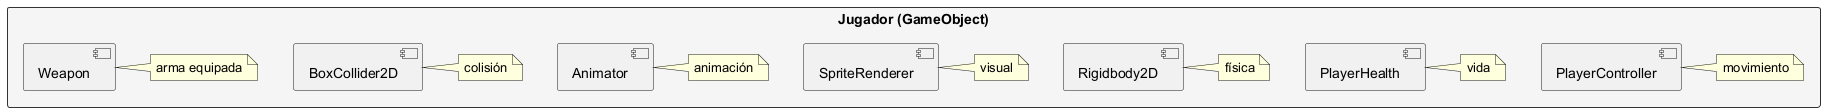
\includegraphics[width=0.95\textwidth]{Figuras/composicion_jugador.png}
\caption{
Diagrama de la composición del jugador. \textit{Elaboración propia.}
}
\label{fig:placeholder-14}
\end{center}
\end{figure}


\textbf{Justificación:} Favorece la composición sobre la herencia. Cada componente encapsula una responsabilidad única (movimiento, vida, física, renderizado), lo que permite reutilizar componentes entre entidades distintas y modificar una funcionalidad sin afectar a las demás. Por ejemplo, el componente \texttt{PlayerHealth} podría reutilizarse en un futuro NPC aliado sin necesidad de heredar de \texttt{PlayerController}.

\subsection{Máquina de estados (\textit{State Machine})}


Como se introdujo en el análisis del estado del arte, el \texttt{GameManager} implementa una máquina de estados. La decisión de diseño responde al siguiente problema:

\textbf{Problema.} El flujo global del juego atraviesa múltiples fases (menú, selección de clase, partida, pausa, fin de partida) con transiciones condicionadas. Sin una estructura explícita, el código del \texttt{GameManager} tendería a acumular variables booleanas (\texttt{isPaused}, \texttt{isGameOver}, \texttt{isInMenu}) cuyas combinaciones serían difíciles de mantener y probar.

\textbf{Alternativa descartada.} Variables booleanas independientes para cada estado. Se descartó porque $n$ booleanos producen $2^n$ combinaciones posibles, la mayoría de las cuales representan estados inválidos (por ejemplo, \texttt{isPaused == true} y \texttt{isGameOver == true} simultáneamente). Una enumeración con seis valores permite exactamente seis estados válidos, eliminando combinaciones ilógicas por construcción.

\textbf{Aplicación en el proyecto:} Control del flujo global del juego en \texttt{GameManager}.

\begin{figure}[H]
\begin{center}
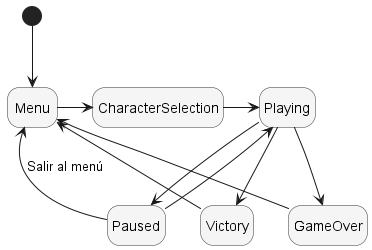
\includegraphics[width=0.95\textwidth]{Figuras/estados_juego.png}
\caption{
Diagrama de los estados del juego. \textit{Elaboración propia.}
}
\label{fig:placeholder-15}
\end{center}
\end{figure}


\textbf{Justificación:} Modela de forma explícita los estados válidos del juego y las transiciones permitidas entre ellos, reduciendo la probabilidad de estados no contemplados y facilitando la comprensión del flujo del juego.

\subsection{Interacción entre patrones: análisis de flujos transversales}


Los patrones descritos en las secciones anteriores no operan de forma aislada, sino que se combinan en cadenas de interacción que atraviesan múltiples subsistemas. A continuación se analizan tres flujos representativos que ilustran cómo la combinación de patrones produce un diseño cohesivo con bajo acoplamiento.

\subsubsection{Flujo 1: Muerte de un enemigo (\textit{Template Method} + \textit{Observer} + \textit{Singleton})}


Cuando un enemigo es eliminado, intervienen tres patrones en cadena. El patrón \textit{Template Method} proporciona el método \texttt{Die()} en la clase base \texttt{Enemy}, que todas las subclases heredan sin sobrescribir. Este método invoca al \texttt{GameManager} -- accesible globalmente mediante el patrón \textit{Singleton} -- a través del método \texttt{NotifyEnemyKilled()}. A su vez, el \texttt{GameManager} emite el evento \texttt{OnEnemyKilled} del patrón \textit{Observer}, al que están suscritos los componentes de interfaz de usuario.

\begin{lstlisting}
// (1) Template Method: Enemy.Die() -- heredado por SlimeGreen, SlimeRed, SlimeBlue
protected virtual void Die() {
    if (isDead) return;
    isDead = true;
    
    // (2) Singleton: acceso global al GameManager
    if (GameManager.Instance != null) {
        int scoreValue = enemyData != null ? enemyData.damage * 5 : 10;
        GameManager.Instance.NotifyEnemyKilled(scoreValue);
    }
    
    if (animator != null && animator.runtimeAnimatorController != null && hasAnimDieTrigger) {
        animator.SetTrigger("Die");
        Destroy(gameObject, 0.5f);
    } else {
        Destroy(gameObject);
    }
}

// (3) Observer: GameManager emite evento que la UI recibe
public void NotifyEnemyKilled(int scoreValue = 10) {
    enemiesKilled++;
    ScoreManager.Instance?.Add(scoreValue);     // Singleton: acceso al ScoreManager
    OnEnemyKilled?.Invoke(enemiesKilled);       // Observer: notifica a la UI
}
\end{lstlisting}


La cadena completa es: \textbf{Template Method} (el esqueleto de \texttt{Die()} se define una sola vez) -> \textbf{Singleton} (acceso al gestor central sin propagación de referencias) -> \textbf{Observer} (desacoplamiento entre la lógica de muerte y la interfaz de usuario). Si se hubiera implementado sin estos patrones, cada subclase de enemigo habría necesitado duplicar la lógica de muerte, mantener una referencia explícita al \texttt{GameManager} (pasada por constructor o asignada en el inspector) y conocer directamente los componentes de UI que deben actualizarse.

\subsubsection{Flujo 2: Ataque del jugador (\textit{Strategy} + \textit{ScriptableObject} + \textit{Singleton})}


Cuando el jugador ataca, intervienen el patrón \textit{Strategy}, el sistema de \textit{ScriptableObjects} y el patrón \textit{Singleton}. El \texttt{PlayerController} invoca \texttt{weapon.Attack()} a través de la interfaz común de la clase base \texttt{Weapon} (\textit{Strategy}), sin conocer si el arma es cuerpo a cuerpo o a distancia. La implementación concreta -- definida en \texttt{MeleeWeapon} o \texttt{RangedWeapon} -- consulta los parámetros del \textit{ScriptableObject} \texttt{WeaponData} para obtener el daño base y, en el caso de las armas a distancia, el prefab del proyectil. El proyectil, a su vez, consulta al \texttt{DamageBoostManager} (\textit{Singleton}) para aplicar las bonificaciones de daño de los tiles de potenciación.

\begin{lstlisting}
// (1) Strategy: el PlayerController no distingue entre tipos de arma
weapon.Attack();    // Polimorfismo: ejecuta MeleeWeapon.Attack() o RangedWeapon.Attack()

// (2) ScriptableObject: el arma consulta sus parametros de un activo externo
public override void Attack() {
    // ...
    projectileScript.damage = weaponData.damage;   // Dato del ScriptableObject
}

// (3) Singleton: el proyectil consulta al gestor de bonificacion
void Start() {
    damage = DamageBoostManager.Instance.GetBoostedDamage(damage);  // Singleton
}
\end{lstlisting}


\subsubsection{Flujo 3: Cambio de estado del juego (\textit{State Machine} + \textit{Observer} + \textit{Singleton})}


La transición de estado del juego ejemplifica la interacción entre la máquina de estados, el patrón \textit{Observer} y el patrón \textit{Singleton}. Cuando el jugador pulsa la tecla de pausa, el \texttt{PauseMenu} accede al \texttt{GameManager} mediante el \textit{Singleton} y solicita un cambio de estado. La máquina de estados del \texttt{GameManager} procesa la transición (modifica \texttt{Time.timeScale}, actualiza la variable \texttt{currentState}) y emite el evento \texttt{OnGameStateChanged} del patrón \textit{Observer}. Todos los componentes suscritos -- incluido el propio \texttt{PauseMenu} que originó la petición -- reaccionan al evento de forma independiente.

\begin{lstlisting}
// (1) Singleton: acceso al gestor central desde cualquier componente
GameManager.Instance.ChangeState(GameState.Paused);

// (2) State Machine: procesamiento de la transicion
public void ChangeState(GameState newState) {
    currentState = newState;
    Time.timeScale = newState == GameState.Playing ? 1f : 0f;
    
    // (3) Observer: notificacion a todos los suscriptores
    OnGameStateChanged?.Invoke(newState);
}

// (4) Suscriptores independientes reaccionan sin acoplamiento
// PauseMenu:
private void OnGameStateChanged(GameState state) {
    EnsureRuntimeUIIfMissing();
    if (pauseMenuPanel == null) return;
    pauseMenuPanel.SetActive(state == GameState.Paused);
}
// GameOverScreen:
private void OnGameStateChanged(GameState state) {
    gameOverPanel.SetActive(state == GameState.GameOver);
}
\end{lstlisting}


Esta interacción demuestra una propiedad arquitectónica: el emisor del evento (\texttt{GameManager}) no conoce ni la cantidad ni la identidad de los suscriptores, lo que permite añadir nuevos componentes reactivos -- por ejemplo, un futuro sistema de audio que silencie la música al pausar -- sin modificar el código del \texttt{GameManager} ni de los suscriptores existentes.
